\documentclass{beamer}

% theme definition
\usetheme{KU}

%\usepackage{natbib}
\usepackage{alltt}
\usepackage{trust}

\usepackage{tikz}
\usetikzlibrary{arrows,shadows}
\usepackage[underline=false]{pgf-umlsd}

\setbeamertemplate{blocks}[rounded][shadow=true]

\setbeamercolor{title}{fg=kublue}
\setbeamercolor{subtitle}{fg=kugray} 
\setbeamercolor{institute}{fg=kugray}
\setbeamercolor{frametitle}{fg=kublue}
\setbeamercolor{frametitle}{bg=white}
\setbeamercolor{framesubtitle}{fg=kugray}
\setbeamercolor{framesubtitle}{bg=white}
\setbeamercolor{item}{fg=black}
\setbeamercolor{subitem}{fg=kugray}
\setbeamercolor{itemize/enumerate subbody}{fg=kugray}
\setbeamercolor{block title}{bg=kublue}
\setbeamercolor{block title}{fg=white}
\setbeamercolor{block body}{bg=sand}
\setbeamercolor{block body}{fg=black}

\usefonttheme{serif}

\newenvironment{fnverbatim}{\begin{alltt}\scriptsize}{\normalsize\end{alltt}}
\newcommand{\mean}[1]{\langle#1\rangle}
\newcommand{\rtime}{\ensuremath{\mathbb{R}^{0\leq}}}

\bibliographystyle{abbrv}

\title{ArmoredSoftware: Trust in the cloud}
\subtitle{Annual Demonstration}

\author{Dr. Perry Alexander, Dr. Andrew Gill, Dr. Prasad Kulkarni,
  Adam Petz, Paul Kline, Justin Dawson, Jason Gevargizian, Leon Searl,
  Edward Komp}

\date{{\color{kugray}January 15, 2015}}

% turns off navigation symbols
\setbeamertemplate{navigation symbols}{}

\institute{
    Information and Telecommunication Technology Center \\
    Electrical Engineering and Computer Science \\
    The University of Kansas \\
    \texttt{palexand@ku.edu,andygill@ku.edu,prasadk@ku.edu}}

\begin{document}

\begin{frame}
  \titlepage
\end{frame}

\begin{frame}
  \frametitle{Outline}
  \tableofcontents
\end{frame}

\section{Introduction and Project Goals}
\subsection{Big Picture}

\begin{frame}
  \frametitle{Program Goal}
  \begin{block}{Trust in the Cloud}
    Provide new capabilities that help establish and maintain
    trustworthy cloud-based application deployment
  \end{block}
\end{frame}

\begin{frame}
  \frametitle{New Capabilities}
  
  \begin{itemize}
  \item Establish trust among cloud components
    \begin{itemize}
    \item trust among cohorts of processes
    \item trust among processes and environment
    \end{itemize}
  \item Promote informed decision making
    \begin{itemize}
    \item data confidentiality can be confirmed
    \item execution and data integrity can be confirmed
    \end{itemize}
  \item Autonomous run-time response and reconfiguration
    \begin{itemize}
    \item responds to attack, failure, reconfiguration, and repair 
    \item response varies based on measurement
    \end{itemize}
  \item Lightweight integration with existing cloud
    \begin{itemize}
    \item targeting TXT, Xen, Linux, and OpenStack infrastructure
    \item user-space measurement and attestation
    \end{itemize}
  \end{itemize}
\end{frame}

\begin{frame}
  \frametitle{High-Level Architecture}
  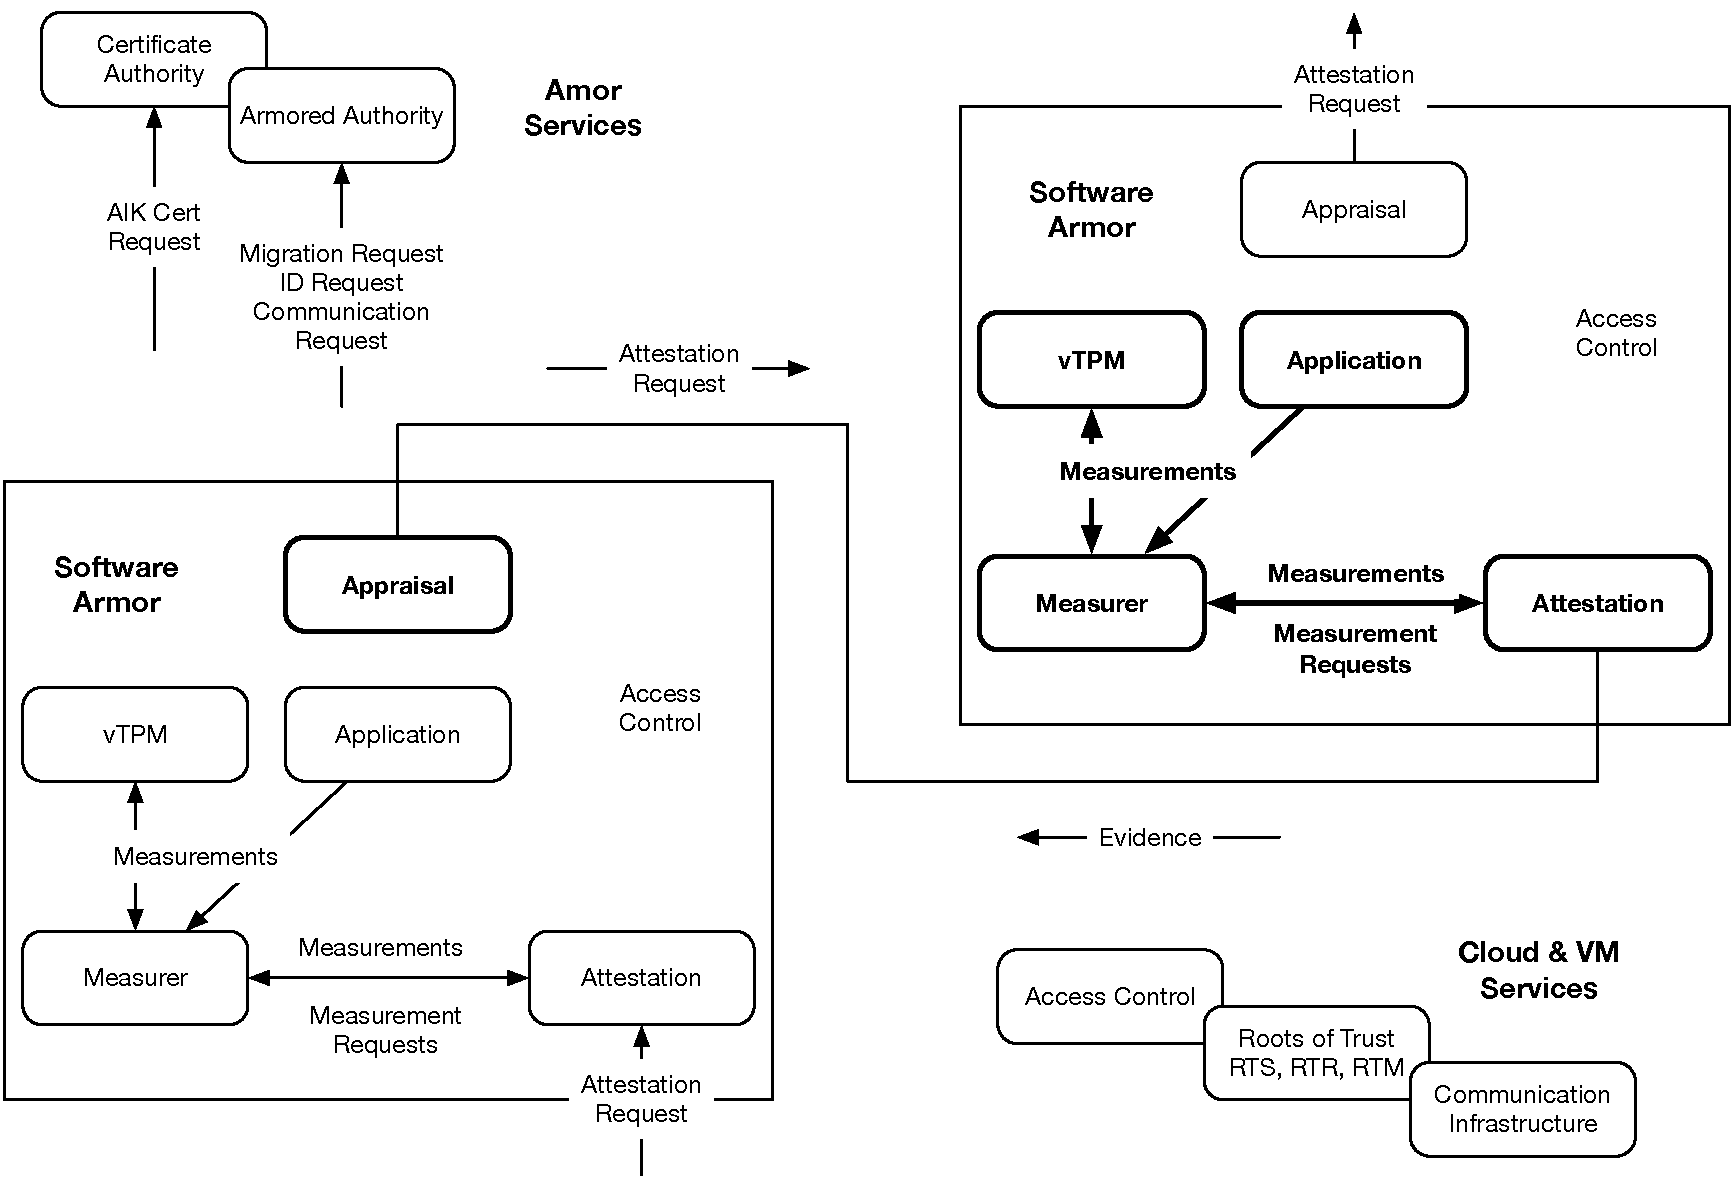
\includegraphics[width=\textwidth]{figures/system.pdf}
\end{frame}

\subsection{Implementation}

\begin{frame}
  \frametitle{Implementation Decisions}

  \begin{itemize}
  \item Standard delivery platform
    \begin{itemize}
    \item Xen+XSM VM infrastructure
    \item OpenStack cloud infrastructure
    \item Fedora, HotSpot JVM, GHC
    \end{itemize}
  \item Standard communication mechanisms
    \begin{itemize}
    \item JSON structures for all exchanged data
    \item \textsl{vchan} for on-platform communication
    \item TCP/IP for off-platform communication
    \end{itemize}
  \item Trusted Computing Group standards compliant
    \begin{itemize}
    \item Trusted Platform Module (TPM) 1.2
    \item TCG vTPM in principle
    \end{itemize}
  \item Executable protocol representation
    \begin{itemize}
    \item protocol fragments as first-class structures
    \item strand space formal semantics
    \end{itemize}
  \end{itemize}
\end{frame}

\section{Prototype demonstration and discussion}

\begin{frame}
  \frametitle{CA-Based Attestation Protocol}
  
  \begin{footnotesize}
  \begin{sequencediagram}
    \newthread[white]{appr}{Appraiser}
    \newinst[1.0]{attest}{Attestation}
    \newinst[1.5]{meas}{Measurer}
    \newinst[1.0]{app}{Application}
    
    \begin{call}{appr}{Request}{attest}{Evidence}
      \begin{callself}{attest}{Protocol Selection}{}
      \end{callself}
      \begin{call}{attest}{Request}{meas}{Value}
        \begin{call}{meas}{Measurement}{app}{Value}
        \end{call}
      \end{call}
      \begin{callself}{attest}{Quote Assembly}{}
      \end{callself}
    \end{call}
    \begin{callself}{appr}{Appraisal}{Execute Decision}
    \end{callself}
  \end{sequencediagram}
  \end{footnotesize}

\end{frame}

\subsection{Refine big picture to current demo}

\begin{frame}
  \frametitle{What We Are Demonstrating}
\end{frame}

\subsection{Protocol Execution}

\begin{frame}
  \frametitle{3-4 Slides on Attestation Protocol Execution}
\end{frame}

\subsection{Appraisal}

\begin{frame}
  \frametitle{1-2 Slides on Appraisal}
\end{frame}

\subsection{Measurement}

\begin{frame}
  \frametitle{3-4 Slides on Measurement}
\end{frame}

\subsection{Communication}

\begin{frame}
  \frametitle{2-3 Slides on Communication Mechanisms}
\end{frame}

\subsection{Demonstration}

\begin{frame}
  \frametitle{Step Through Demonstration}
\end{frame}

\section{Short term goals and milestones}

\begin{frame}
  \frametitle{Goals and Milestones for 2015}

  \begin{itemize}
  \item Push to the cloud
  \item Establish roots of trust and trust argument
  \item Executable protocol representation and protocol semantics
  \item Operational, integrated vTPM prototype
  \item Name Server / Certificate Authority prototype
  \item More capable measurement
  \item Downloadable demonstration
  \end{itemize}
\end{frame}

\section{Questions and guidance}

\begin{frame}
  \frametitle{Questions and Guidance}

  \begin{itemize}
  \item What problems are interesting?
  \item What problem would be a nice attention grabber?
  \item What should we be watching and integrating with?
  \end{itemize}
\end{frame}

\nocite{Coker::Principles-of-R,Haldar:04:Semantic-Remote,Fabrega:1999aa}

\begin{frame}
  \frametitle{References}
  \bibliography{demo14}
\end{frame}

\end{document}

